\documentclass[11pt,nonblindrev,fleqn]{article}
\pagestyle{plain}

%\include{epsf}
\include{amsfonts}
\usepackage{graphicx}
\usepackage{amssymb,amsmath}
\usepackage{mathrsfs,threeparttable,lscape,subfigure,float,booktabs,enumerate,multirow,epstopdf,longtable}
\usepackage{algorithm,algorithmic,xcolor}
%\usepackage{hyperref,color}
%hyperlink colour set
\usepackage[colorlinks,linkcolor=blue,anchorcolor=blue,citecolor=blue]{hyperref}

%\usetikzlibrary{shapes,snakes}
%\newcommand{\USA}{\USAmap}

% Natbib setup for author-year style
\usepackage{natbib}
 \bibpunct[, ]{(}{)}{,}{a}{}{,}%
 \def\bibfont{\small}%
 \def\bibsep{\smallskipamount}%
 \def\bibhang{24pt}%
 \def\newblock{\ }%
 \def\BIBand{and}%

% Set page dimensions
\evensidemargin -.5in
\oddsidemargin -.5in
\textwidth 7.5in
\topmargin -0.5in
\textheight 9in

\newcommand{\singlespace}{\renewcommand{\baselinestretch}{1}\small\normalsize}
\newcommand{\doublespace}{\renewcommand{\baselinestretch}{1.5}\small\normalsize}


\begin{document}


\singlespace

\begin{titlepage}
\title{A branch-and-cut-and-price algorithm for large-scale service network design considering heterogeneous fleets and service capacity decision}
\author{
	Zujian Wang \\
	\small{Department of Industrial Engineering} \\
	\small{Tsinghua University, Beijing 100084, China} \\
	%\small{200 West Packer Ave., Mohler Lab} \\
	%\small{Bethlehem, PA, 18015, USA} \\
	%\small{P: 610 758 6696 F: 610 758 4886} \\
	\small{\tt wang-zj14@mails.tsinghua.edu.cn} \\
	}
\date{} % version 11
\end{titlepage}
\maketitle

%\newpage

\abstract{
Service network design addresses decisions related to selecting transportation services and distributing origin-to-destination commodity flow. In this paper, we consider the usage of heterogeneous fleets to provide transportation services. The amounts of fleets employed by each service decide its capacity. We propose both arc-based and cycle-path based models to formulate the problem.  A branch-and-cut-and-price algorithm is presented to solve the problem. The method includes pricing and cutting techniques, as well as a local search algorithm to obtain upper bound. The computation study indicates the efficiency of the proposed algorithm.
}

\vspace{.25in}

\noindent {\bf Keywords:} a heterogeneous fleet; column generation;



%\newpage

%%%%%%%%%%%%%%%%
% INTRODUCTION %
%%%%%%%%%%%%%%%%

\doublespace
%\singlespace
\section{Introduction}
Freight transportation plays an increasingly important role because of rapid development of e-commerce. Carriers are facing tremendous pressure from growing competition and start to pay more attention to optimize their transportation network. Service network design (SND) formulations address issues related to the tactical planning for consolidation-based freight transportation systems. Specifically, such formulations make decisions on selecting transportation services and distributing origin-destination (O-D) commodity flow.
% remain to change
Network links represent services with operational assets (e.g. vehicles, drivers, power units, etc.) in SND formulations. Asset management concentrates on the operation and schedule of assets which  The main goal of research on such issue is to acquire an efficient allocation and utilization of assets under the circumstance of satisfying the origin-destination demand.

The models with asset management introduced in the literature only take single type of vehicles into consideration.

It is more realistic to employ heterogeneous fleets in application to freight transportation system for carriers when providing transportation services. However, only a small amount of literature is devoted to considering heterogeneous fleets, e.g. \cite{Kim1999Multimodal} and \cite{Li2016Design}. Since service network design problem is NP-hard, it is difficult to find a feasible solution of large-scale instance. However, in real-life application, carriers are confronted with huge transportation network and need efficient algorithms to reduce costs.

Our goal of this paper is to address this issue about heterogeneous fleets and propose two kinds of formulations. And a hybrid algorithm combining both exact and heuristics techniques is introduced to obtain high-quality feasible solutions in a short time. Meanwhile, the algorithm provide lower bounds on each instance to show how far the solution is away from the optimal value.

The outline of this paper is as follows. In Section 2, a brief literature review is elaborated. We describe the problem and propose both arc-based and cycle-path formulations in Section 3. Section 4 is devoted to the proposed hybrid algorithm, whereas experimental results is presented in Section 5. Concluding remarks is given in Section 6.

\section{Literature review}
% 1.asset management 2.arc, cycle structure models 3.large-scale 4.heterogenerous fleets
Service network design(SND) contains the tactical planning decisions on selecting transportation services to satisfy O-D demands which is generally formulated as fixed-cost capacitated multicommodity network design problem (CMND), see \cite{Magnanti1984Network}, \cite{Minoux1989Networks}. In addition to scheduling services and distributing flow, asset management is marginally considered in \cite{Crainic2000Service}, \cite{Smilowitz2002Deferred} and \cite{crainic2003long}. Since carriers attach increasing importance to utilize assets economically and efficiently, SND with asset management attracts increasing attention in the literature \citep{Andersen2009bService,Teypaz2010A}.   Afterwards design-balanced constraints are proposed by \cite{Pedersen2009Models}, which state that the number of assets entering each terminal must equal the number of leaving. The design-balanced constraints induce a cyclic structure for the assets movements to complete service operations and flow distribution.

With respect to the way to formulate SND, it is general to introduce arc-based formulation in the literature. While \cite{Andersen2009bService} present four alternative formulations and analyze strengths and weaknesses of each formulation. The experimental results show that formulations based on cycle variables outperform other formulations in both solution quality and time. However, the amount of generated cycles grows exponentially and requires more efficient enumeration algorithm. Consequently, \cite{Andersen2011Branch} propose an efficient branch-and-price scheme for the cycle-based formulation to avoid the enumeration of cycles. Their algorithm contains two subproblems for the dynamical construction of paths for commodities and cycles for vehicles.

Since the SND problem is NP-hard, heuristic methods are preferred choices with respect to the large scale of instances. \cite{Pedersen2009Models} present a two-phase tabu search meta-heuristic framework for the arc-based formulation. The proposed algorithm includes exploration phase to build neighborhoods and feasibility phase to implement an infeasibility-monitoring procedure for reaching good feasible solutions. \cite{Teypaz2010A} present a three-step decomposition heuristic to solve large-scale freight transportation formulation and build comprehensive solutions for real-life size instances. \cite{VuDucToulouse} propose a three-phase meta-heuristic method combining neighbourhood-based and exact methods. Additionally, computational results on large-scale benchmark instances indicate the efficiency of the algorithm. Another meta-heuristic combining a cutting-plane scheme to obtain lower bound and a variable fixing procedure to cut down the dimension of the problem is introduced in \cite{Chouman2015Cutting}. \cite{Crainic2016Service} propose a new service network design model with resource constraints and design a solution approach combining column generation and slope scaling methods to find high-quality solutions.

A single asset type is considered in the aforementioned literature. As for heterogeneous assets, especially multiple types of vehicles, \cite{Kim1999Multimodal} introduce three different formulations and two sets of valid inequalities. However, no efficient algorithm is mentioned to solve those formulations in that paper. \cite{Li2016Design} propose a tabu search based meta-heuristic to solve arc-based formulation for design-balanced capacitated multicommodity network design with heterogeneous vehicles. The amounts of each type of vehicle used by each service are not decided explicitly in their paper.

Our research makes the following contributions to the literature: First, we present both arc-based and cycle-path formulations for service network design considering heterogeneous fleets. Second, a hybrid algorithm including column generation, cutting plane and local search methods is introduced. Moreover, the proposed algorithm provides high-quality both lower bounds and feasible solutions for large-scale instances efficiently.

\section{Problem statement and model formulation}
In this section, we introduce two kinds of model formulations to describe the problem.

\subsection{Problem description}
Transportation carriers need a sufficient system to support their tactical planning. They tend to employ heterogeneous fleet to increase the loading rate under the condition of satisfying the time requirements of each commodity. Under the assumption of known demand at each terminal, they need to schedule the heterogeneous fleet including the routing terminals, the arriving and departure time at each terminal.

To solve the problem, we work with cyclic time-space network $\mathscr{G}=(\mathscr{N},\mathscr{A})$ which is shown in Fig. \ref{Fig1}. The schedule length is the length of time (e.g. a week) during which the scheduling pattern is employed. We assume the schedule length is divided into $\mathscr{T}=\{1,2,...,TMAX\}$ time periods. Physical terminals at different time period is formulated as different nodes in time-space network. Therefore, the set of nodes denoted by $\mathscr{N}$ is defined as $\mathscr{N}=\mathscr{T}\times \mathscr{P}$, where $\mathscr{P}$ represents the set of physical terminals.
\begin{figure}[H]
\setlength{\abovecaptionskip}{-5pt}
\setlength{\belowcaptionskip}{-5pt}
\centering
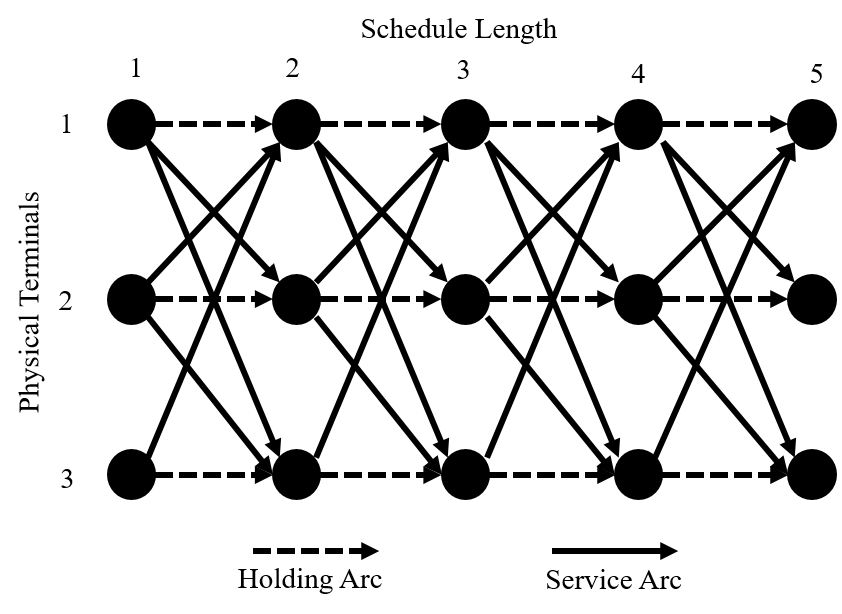
\includegraphics[width=0.5\linewidth]{F1.png}
\caption{\small Time-space diagram for cyclic transportation service schedule}
\label{Fig1}
\end{figure}

\begin{figure}[H]
\setlength{\abovecaptionskip}{-5pt}
\setlength{\belowcaptionskip}{-5pt}
\centering
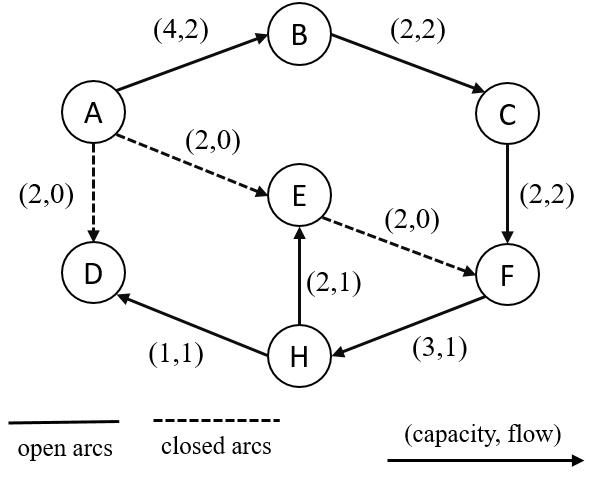
\includegraphics[width=0.5\linewidth]{F2.png}
\caption{\small Time-space network with heterogeneous fleet operating}
\label{Fig2}
\end{figure}

In our problem setting there are two types of arcs in the set $\mathscr{A}$. The first is the horizontal lines between nodes called holding arcs, which represent vehicles and commodities wait at the same terminal. The second is the service arcs representing the operation of a transportation service between two different terminals at a specific time period. We denote the set of the holding arcs by $\mathscr{H}$ and the service arcs by $\mathscr{S}$, thus we have $\mathscr{A}=\mathscr{H}\cup \mathscr{S}$.

One of the feature of our formulation is taking heterogeneous fleet into into consideration. The time-space network with heterogeneous fleet operating is shown in Fig. \ref{Fig2}. Under this assumption, the amount of different type of vehicles should be figured out on each arc. In Fig. \ref{Fig2} the number besides each arc denotes the number of particular type of vehicles. At each node in the set of $\mathscr{N}$ the numbers of same type of vehicle entering and leaving equals. The set of fleet type is denoted by $\mathscr{F}$.

\subsection{Arc-based formulation}
A set of commodities $K$ represents different products that require to be transited from particular origin to destination terminals. Each commodity $k\in K$ requires a certain quantity demand $d_k$. The fixed cost of selecting and operating transportation service $(i,j)\in A$ by vehicle type $f\in F$ is denoted $h_{ij}^f$. The unit flow cost on each arc $(i,j)$ with respect to commodity $k\in K$ is denoted $c_{ij}^k$. The capacity of vehicle type $f$ is denoted by $u^f$. We define $N_i^+:\{j\in N:(i,j)\in A\},N_i^-:\{j\in N:(j,i)\in A\}$. For each commodity $k$ and node $i$, define
\begin{equation*}
\omega_i^k= \left\{
\begin{aligned}
d_k &  & if \quad i=o(k) \\
-d_k &  & if \quad i=d(k) \\
0 &  & otherwise
\end{aligned}
\right.
\end{equation*}

We define two sets of decision variables:
\begin{itemize}
  \item Continuous variable: $x_{ij}^k$ denotes the amount of commodity $k\in K$ that flows on arc $(i,j)\in A$;
  \item Integer variable: $y_{ij}^f$ indicates the amount of fleet type $f\in F$ that provide services on arc $(i,j)\in A$.
\end{itemize}

The model is formulated as follows:
\begin{align}
  \min & \sum_{k\in K}\sum_{(i,j)\in A} c_{ij}^k x_{ij}^k + \sum_{f\in F}\sum_{(i,j)\in A}h_{ij}^f y_{ij}^f    \label{objA}  \\
  \rm{s.t.} \nonumber  \\
         &  \sum_{j\in N_i^+}x_{ij}^k - \sum_{j\in N_i^-}x_{ji}^k = w_i^k     \quad     \forall i\in N, \forall k\in K,     \label{demandA}  \\
         &   \sum_{j\in N_i^+}y_{ij}^f - \sum_{j\in N_i^-}y_{ji}^f = 0  \quad     \forall i\in N, \forall f\in F,   \label{dbA} \\
         &   \sum_{k\in K}x_{ij}^k \leq \sum_{f\in F}u^f y_{ij}^f  \quad  \forall (i,j)\in A,   \label{capacityA} \\
         &    x_{ij}^k \geq 0  \quad  \forall (i,j)\in A, \forall k\in K,   \label{xA} \\
         &   y_{ij}^f \in Z_0^+  \quad  \forall (i,j)\in A,\forall f\in F, \label{yA}
\end{align}

% remain to modify
The objective function (\ref{objA}) minimizes the total cost calculated as the sum of the flow costs on arcs plus the fixed costs for selecting and operating transportation service with respect to different types of vehicles. Constrains (\ref{demandA}) give the flow conversation relations for each commodity and each node. Equations (\ref{dbA}) are the design-balance constraints, which indicate that the total number of each type of vehicle entering a node equals the total number of each type of vehicle leaving that node. Through constrains (\ref{capacityA}), we enforce service capacity restrictions on each arc. Finally, Constrains (\ref{xA}) and (\ref{yA}) give variable-type restrictions.

\subsection{Cycle-path formulation}
Cycle-path based service network design formulation, presented in \cite{Andersen2011Branch} has been proved outperforming other form of formulation. We define heterogeneous vehicle design-cycle $q\in Q^f$ consisting of a sequence of paths $p\in P^k$ which transit commodities $k\in K$ by heterogeneous fleets $f\in F$. The fixed cost of cycle $q$ provided transportation services by vehicle type $f\in F$ is denoted $h_q^f$. The unit flow cost of path $p$ with respect to vehicle type $f\in F$ is denoted $c_p^k$.

We define two sets of decision variables:
\begin{itemize}
  \item Cycle integer variables: $y_q^f$ denotes the amount of vehicles used by each cycle;
  \item Path continuous variables: $x_p^k$ denotes the volume of specific commodity on path $p$ with respect to vehicle type $v$.
\end{itemize}

\begin{align}
  \min &    \sum_{f\in F}\sum_{q\in Q^f}h_q^f y_q^f  +   \sum_{k\in K}\sum_{p\in P^k}c_p^k x_p^k  \label{objCP}    \\
         & \rm{s.t.} \nonumber \\
         &     \sum_{k\in K}\sum_{p\in P^k}\delta_{ij}^p x_p^k \leq  \sum_{f\in F}\sum_{q\in Q^f}u^f \alpha_{ij}^q y_q^f      \quad \forall (i,j)\in A \label{capacityCP}\\
         &     \sum_{p\in P^k}x_p^k = d^k      \quad       \forall k\in K  \label{demandCP}    \\
         &      x_p^k \geq 0        \quad       \forall p\in P^k,\forall k\in K     \label{xCP} \\
         &      y_q^f \in Z_0^+     \quad       \forall q\in Q^f, \forall f\in F    \label{yCP}
\end{align}

The objective function (\ref{objCP}) minimizes the total cost calculated as the sum of the flow costs on paths plus the fixed costs for selected cycles with respect to specific type of vehicle.Through constrains (\ref{capacityCP}), we enforce service capacity restrictions on each arc. Constrains (\ref{demandCP}) ensure demand satisfaction corresponding to the flow conservation equations for each commodity.  Finally, Constrains (\ref{xCP}) and (\ref{yCP}) gives variable-type restrictions.

\section{Solution method}
Since the service network design problem is NP-hard, the exact algorithm is difficult to solve the large scale instances optimally. Heuristics and metaheuristics are the common choices in real-life application. But the drawback of heuristics algorithm is that the results cannot be evaluated by lower bound. Therefore we propose a branch-and-cut-and-price method combining the exact and the heuristics algorithm to solve the problem. The exact part mainly contains column generation and cutting plane method to obtain lower bound. The heuristic method uses local search and tabu search techniques to find feasible solutions at nodes on search tree.

\subsection{Column generation}
\cite{Andersen2011Branch} proposed a branch-and-price algorithm for service network design with asset management constrains. However heterogeneous fleets are not taken into consideration in the literature. This paper aims to be devoted to filling the gap.The linear relaxation of the cycle-path formulation constitutes the master problem(MP) which is solved by the column generation approach. The number of variables in the MP is exponentially increasing thus it is necessary to concentrate on a restricted master problem(RMP) which contain only a subset of variables in the MP. The column generation approach generates columns dynamically until no additional column can be found.

\subsubsection{Restricted master problem}
The restricted master problem(RMP) works on subsets of cycles and paths. Dual variables $\eta_{ij}$ and $\omega_k$ are associated with constrains (\ref{capacityCP}) and (\ref{demandCP}) respectively.To search for columns whose reduced cost is negative but are not included in the RMP, we solve the linear relaxation of RMP by use CPLEX as the LP-solver. The dual variable values in the solution of the RMP are past on to the subproblem for generating new columns. We initialize the RMP with a limited set of cycle-path variables. To avoid demand constraints violation, the RMP includes path-vehicle flow decision variables entirely.
\subsubsection{Cycle subproblem}
A cycle satisfying design-balance requirements consists of paths providing services $s\in \mathscr{S}$ by the same type of vehicle. Thus the objective of the cycle-selection subproblem is to find cycle-vehicle variables $y_{qv}$ with negative reduced cost which is given by:
\begin{align}
RC_{fq} = h_q^f + \sum_{(i,j)\in A} u^f \alpha_{ij}^q \eta_{ij} = \sum_{(i,j)\in q} (h_{ij}^f + u^f \eta_{ij})
\end{align}

We initialize the network with a subset of cycles to avoid constraints violation and ensure RMP being feasible. Each time we add a certain number of cycle-vehicle variables with least reduced cost to the RMP.

\subsubsection{Path subproblem}

\begin{align}
RP_{kp} = c_p^k - \sum_{(i,j)\in A} \delta_{ij}^p \eta_{ij} - \sigma_k = \sum_{(i,j)\in p} (c_{ij}^k - \eta_{ij}) - \sigma_k
\end{align}

\subsection{Cutting plane}
The generation of valid inequalities can help strength the lower bound obtained by column generation. We introduce two sets of valid inequalities including strong inequalities and cutset inequalities.

\subsubsection{Strong inequalities(SI)}
SI have been widely used to improve the quality of the LP lower bound. SI added to the model in our paper are defined as
\begin{align}
  x_{ij}^k \leq d^k \sum_{f\in F} y_{ij}^f      \quad       \forall (i,j)\in A, \forall k\in K.
\end{align}

\subsubsection{Cutset inequalities(CI)}
CI have been used by \cite{Chouman2015Cutting} to strength the lower bound. As for heterogeneous fleet, the CI have been presented by \cite{Kim1999Multimodal} which are defined as
\begin{align}
    \sum_{f\in F}u^f Y_{S,\bar{S}}^f \geq  D_{S,\bar{S}}
\end{align}

where we define cutset $(S,\bar{S})$ by partitioning the node set $N$ into any nonempty subset $S$ and its complement $\bar{S}=N\backslash S$. An arc $(i,j)$ that connects node $i$ in $S$ to node $j$ in $\bar{S}$  belongs to the cutset $(S,\bar{S})$. Let $Y_{S,\bar{S}}^f$ denote the total amount of type $f$ vehicles used on the cutset $(S,\bar{S})$ arcs, i.e., $\sum_{(i,j)\in (S,\bar{S})} y_{ij}^f$ for the arc-based formulation and $\sum_{q\in Q^f}\sum_{(i,j)\in (S,\bar{S})} \alpha_{ij}^q y_q^f $ for the cycle-path formulation. Let $D_{S,\bar{S}}$ denote the aggregate demand of all commodities with their origin in$S$ and destination in $\bar{S}$. CI ensure the total demand that must flow from $S$ to $\bar{S}$ will be satisfied by enough capacity on the arcs of $(S,\bar{S})$.

In general, the LP solution will not violate CI. Therefore, we strength CI by using a integer rounding procedure to produce $Chv\acute{a}tal$-$Gomory$ (C-G) cuts.
\begin{align}
  \sum_{f\in F} \left( \left \lceil \frac{u_f}{u_l} \right \rceil Y_{S,\bar{S}}^f  \right)  \geq \left\lceil \frac{D_{S,\bar{S}}}{u_l} \right\rceil  \quad   \forall l\in F
\end{align}
% prove???
\subsection{Local search}
Since the application of SND employing heterogeneous fleets by logistics enterprises will deal with large scale of data, it is necessary to present efficient algorithms to find high-quality feasible solutions efficiently. To satisfy the need of solving large scale of instances, we propose a two-stage heuristics algorithm to find feasible solutions.

At each node on the searching tree, the column generation method will provide the value of $x_{ij}^k$ and $y_{ij}^f$. The arc subset $A_1$ includes arcs with nonzero flow on it. Another arc subset $A_2$ includes arcs with nonzero fleets on it. It is easy to find that $A_1\subseteq A_2$ because of the capacity constraints. The values of $\sum_{(i,j)\in A_2}u^f y_{ij}^f $ decide the arc capacity $u_{ij}$ in $A_1$.

\subsubsection{Stage 1: capacitated multi-commodity minimum cost flow problem (CMCF)}
Without considering the design-balance constraints, the capacitated multi-commodity minimum cost flow problem (CMCF) is obtained for given arc capacity. The solutions of the CMCF  determine the flow distribution of each commodity on each arc $(i,j)\in A_1$.
\begin{align}
   \min& \sum_{(i,j)\in A_1}\sum_{k\in K} \bar{c}_{ij}^k x_{ij}^k     \\
   \rm{s.t.} & \nonumber \\
         &  \sum_{j\in N_i^+}x_{ij}^k - \sum_{j\in N_i^-}x_{ji}^k = w_i^k     \quad      \forall i\in N, \forall k\in K,  \\
         &  \sum_{k\in K} x_{ij}^k \leq u_{ij}      \quad    \forall (i,j)\in A_1,  \\
        &  x_{ij}^k \geq 0   \quad    \forall (i,j)\in A_1, \forall k\in K.
\end{align}
After solving the CMCF and redistributing the flow on each arc, the arcs without flow are removed from $A_1$.

\subsubsection{Stage 2: fleet assignment problem (FAP)}
After the flow distribution of origin-to-destination commodities has been completed, we need to assign heterogeneous fleets to provide transportation services. Let $\Omega_{ij}$ be the total flow of all commodities distributed on arc $(i,j) \in A_2$, which equals $\sum_{k\in K}\bar{x}_{ij}^k$. The mathematical formulation of Stage 2 defined on arc set $A_2$ is as follow:
\begin{align}
  \min & \sum_{f\in F}\sum_{(i,j)\in A_2} h_{ij}^f y_{ij}^f \\
    \rm{s.t.} & \nonumber \\
     & \sum_{j\in N_i^+}y_{ij}^f - \sum_{j\in N_i^-}y_{ji}^f = 0     \quad      \forall i\in N,\forall f\in F  \\
     & \sum_{f\in F} u^f y_{ij}^f \geq \Omega_{ij}      \quad       \forall (i,j)\in A_2   \label{cap} \\
     & y_{ij}^f \in Z_0^+       \quad       \forall (i,j)\in A_2, \forall f\in F
\end{align}
Constraints (\ref{cap}) ensure each service arc will provide sufficient vehicle capacity for the total flow.

\subsubsection{Cycle-based neighborhoods}
To improve the upper bound, we introduce cycle-based neighborhoods to search for better feasible solutions. The cycle-based neighborhoods was first proposed by Crainic to solve fixed-charge capacity multicommodity network design.

\section{Numerical experiments and analyses}
The computation study is implemented in C++, using CPLEX 12.63 as the MIP-solver. All experiments are performed using a computer with four 64-bit 2.4 GHz Intel Core processors and 4 GB of RAM, running Window 10.

\section{Conclusion}

\section*{Acknowledgments}

This work was supported by the National Natural Science Foundation of China
\bibliographystyle{ormsv080} % outcomment this and next line in Case 1
\bibliography{References} % if more than one, comma separated
\end{document}
